\fancyhead[LE,RO]{Langmuir isotherm of a solid adsorbent}
\fancyhead[LO,RE]{\thesection}
\fancyfoot[LE,RO]{\thepage}
\fancyfoot[RE,LO]{\emph{Physical chemistry lab. practice for pharmacy students}}

%\setcounter{section}{7}
\section{Using the Langmuir isotherm to calculate the maximal adsorption capacity of a solid adsorbent}
\subsection{Introduction}

Adsorption is a physicochemical process, during which atoms, ions or molecules adhere to a surface.
The result is a thin layer of the adsorbate that is formed on the adsorbent surface (Fig. \ref{fig:adsorption}).
\begin{SCfigure}[][b]
\centering
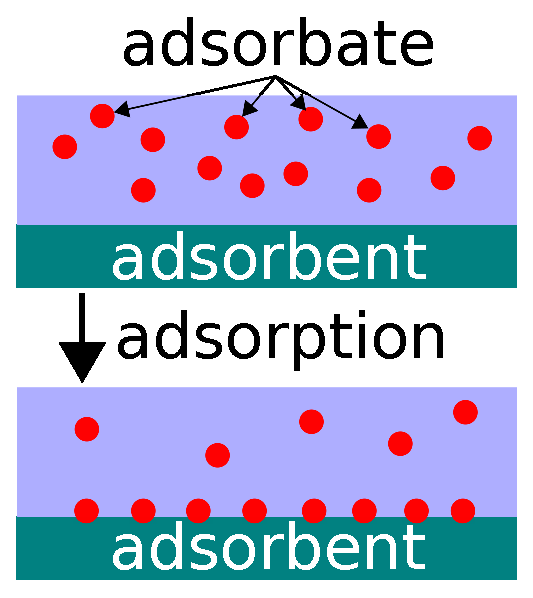
\includegraphics[width=0.25\textwidth]{adsorption.eps}
\caption{During adsorption, a thin adhered layer of the adsorbate is produced on the surface of the adsorbent.}
\label{fig:adsorption}
\end{SCfigure}
The original media from which the adsorbate originates can be gas or liquid.
The reverse process is called desorption.
Adsorption is an important process, and it is present in many areas of everyday life, industry, research, pharmacy.
It is an important step -- among many -- in heterogeneous catalysis, water treatment, removal by activated carbon.
Adsorption by activated carbon is used to remove toxins or unwanted dangerous substances from the gastrointestinal tract after poisonings.
Adsorption can be used in pharmaceutical industry to modulate the rate at which specific components are being released. 
It is the basis of many types of chromatography.

The first theoretical model to describe adsorption was developed by Irving Langmuir:

\begin{equation}
\label{eq:langmuir1}
        \theta
        =
        \frac
                {K p}
                {1 + K p} 
\end{equation}

It is called the \emph{Langmuir isotherm}, and its plot can be seen in Fig. \ref{fig:langmuir}. $\theta$ is the \emph{fractional coverage}, $K$ is $k_d/k_a$, the ratio of the rate of desorption and adsorption. $p$ is the partial pressure of the adsorbate.

\begin{figure}
\centering
\begin{tikzpicture}
\begin{axis}[xtick=\empty, xmin=0,xmax=10,ymin=0,ymax=1.1,xlabel={$c$}, ylabel={$\theta$},no markers,samples=50]
        \addplot[domain=0:10, black] {x/(x+1)};
        \draw [color=red, dashed] (0,100) -- (100,100);
        \draw [color=red, dashed] (10,0) -- (10,50);
	\draw [color=red, fill=red] (10,50) circle [radius=0.1cm];
	\draw [color=red, dashed] (0,50) -- (10,50);
\end{axis}
\end{tikzpicture}
\caption{The Langmuir isotherm. Red dot: $K$, the \emph{half-saturation constant}. $\theta$ eventually reaches 1 (maximal coverage), as $c$ approaches infinity. In practice, maximal coverage is reached much sooner.}
\label{fig:langmuir}
\end{figure}

This equation was derived to describe the adsorption of gases at solid surfaces. However, it also describes the adsorption of a solute from a solution, if the solvent has little or no adsorption to the adsorbent, compared to the solute. After replacing the partial pressure $p$ and multiplying both sides with the \emph{maximal adsorption capacity} $n_{max}$ we get:

\begin{equation}
\label{eq:langmuir2}
        n
        =
        n_{max}
	\frac
                {c}
                {c + K_{half}} 
\end{equation}

where $c$ is the equilibrium concentration of the adsorbate in the solution, $K_{half}$ is the \emph{half-saturation constant}, that equals to $1/K$. The half-saturation constant is the equilibrium concentration of the adsorbate, when half of the available surface is covered, so $\theta = 0.5$. Note that if $c = K_{half}$, then $c/(c + K_{half})$ is $1/2$ and therefore $n = 0.5\, n_{max}$. 

Specific adsorbance ($n^*_{max}$) is the amount of adsorbate adsorbed by 1 g of adsorbent. Its unit is mol/g. The maximal specific adsorption capacity of an adsorbent can be determined from the linearized form of Eq. \ref{eq:langmuir1}:

\begin{equation}
\label{eq:langmuir2}
        \frac{1}{n^*}
        =
        \frac{1}{n^*_{max}}
	+
	\frac{K'}{c}
\end{equation}

If we plot $1/n^*$ as a function of $1/c$, then the $y$-interception will be $1/n^*_{max}$. Determining it is the goal of the practice.

\subsection{Practice procedures}

Prepare a dilution series from known concentration methylene blue stock solution. The series should feature the following concentrations: $2\cdot10^{-4}$, $10^{-4}$, $5\cdot10^{-5}$, $2\cdot10^{-5}$, $10^{-5}$, $5\cdot10^{-6}$ M. Use 50 ml volumetric flasks to prepare the solutions. Record a spectrum of the $2\cdot10^{-5}$ solution, and determine the absorption peak in the visible range. Measure the absorbance of all the solutions. This dataset will be used to prepare the calibration curve.

Pipette 25--25 ml from each solution into a 100 ml Erlenmeyer flask. Put 0.3--0.5 g of adsorbent into each of flasks. The mass should be known in each case. The absorbent will be cellullose (filter paper or cotton swab) on the practice.
Shake the solutions for 30 minutes, then filter them, and measure their absorbance.

Calculate the adsorbed amount, and prepare the $1/n^*$--$1/c$ plot based on Eq. \ref{eq:langmuir2}. Correct for the differences in adsorbent mass by using the specific adsorbance.
After doing a linear regression (line fitting) on the dataset, use the $y$--interception to calculate $n^*_{max}$. 

%Written, updated and translated by András Kiss in 2017.
